\section{Conceptos básicos Android}

% You can reveal the parts of a slide one at a time
% with the \pause command:
\begin{frame}{Conceptos básicos Android}
  \begin{itemize}
    \item {\textbf{View:} Representa el componente básico en el que se apoyan todos los elementos que construyen una interfaz. Todos los elementos que generan interfaces heredan de la clase \texttt{\href{http://developer.android.com/reference/android/view/View.html}{View}}
    \pause
    }

  \item<2-> {
    \textbf{Activity:} Encargada de mostrar la interfaz de usuario e interactuar con él. Responden a los eventos generados por el usuario (pulsar botones etc). Heredan de la clase \href{http://developer.android.com/reference/android/app/Activity.html}{\texttt{Activity}}.
  }
  \item<3-> { \textbf{Services:} No tienen interfaz visual y se ejecutan en segundo plano, se encargan de realizar tareas que deben continuar ejecutandose cuando nuestra aplicación no está en primer plano. Todos los servicios extienden de la clase \texttt{\href{http://developer.android.com/reference/android/app/Service.html}{Service}}
  }
  \end{itemize}
\end{frame}

\begin{frame}{Conceptos básicos Android}
  \begin{itemize}
  \item{
    \textbf{Content Provider:} Ponen un grupo de datos a disposición de distintas aplicaciones, extienden de la clase ContentProvider para implementar los métodos de la interfaz, pero para acceder a esta interfaz se ha de usar una clase llamada ContentResolver.
    \pause
  }
  \item<2-> {
    \textbf{BroadcastReceiver:} Simplemente reciben un mensaje y reaccionan ante él, extienden de la clase BroadcastReceiver, no tienen interfaz de usuario, pero pueden lanzar Actividades como respuesta a un evento o usar NotificationManager para informar al usuario.
  }
  % or you can use the \uncover command to reveal general
  % content (not just \items):
  \item<3-> {
    \textbf{Intent:} Permite realizar la comunicación y transferencia de datos entre objetos de la clase Activity o Service. También permite iniciar otras Activities o lanzar otras aplicaciones.
  }
  \end{itemize}
\end{frame}

\section{Hola Mundo}

\subsection{Crear el proyecto}

\begin{frame}{Crear el proyecto}
\begin{block}{Pasos a realizar}
En Android Studio, File » New Project.
\end{block}
\end{frame}

\subsection{Componentes del proyecto}

\begin{frame}{Componentes del proyecto}
\begin{block}{}
Los proyectos de Android siguen una estructura fija de carpetas que debemos respetar.
\begin{figure}[H]
\centering
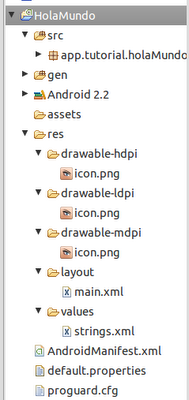
\includegraphics[scale=.3]{./img/estructuraCarpetas.png}
\end{figure}
\end{block}
\end{frame}

\subsubsection{Carpeta Res}

\begin{frame}{Carpeta Res}
\begin{block}{}
Ésta es una de las carpeta que más se va a usar junto con \texttt{src}. Se compila y se generan referencias en la clase \texttt{R}, para acceder a ellos desde código. Están escritos en \texttt{XML}.
\pause
\end{block}
\begin{itemize}
    \item<2-> \texttt{anim}: Definición de Animaciones.
    \item<3-> \texttt{color}: Definición de colores
    \item<4-> \texttt{drawable}: Ficheros bitmap(.png, .9.png, .jpg, .gif) o XML con contenidos que se dibujarán (fondos, botones etc).
    \item<5-> \texttt{layout}: Definen la capa de interfaz de usuario
    \item<6-> \texttt{menu}: Definición de los menús de la aplicación
    \item<7-> \texttt{raw}: Binarios que no se pueden colocar en las otras carpetas.
    \item<8-> \texttt{values}: Definición de estilos, cadenas de texto para Localización etc.
    \item<9-> \texttt{xml}: Ficheros XML que pueden ser accedidos en tiempo de ejecución
\end{itemize}
\end{frame}

\begin{frame}[fragile]{Hola Mundo}
\begin{block}{}
\begin{javacode}
    @Override
    protected void onCreate(Bundle savedInstanceState) {
        super.onCreate(savedInstanceState);

        /**
         * Método encargado de “inflar” la actividad.
         * Inicializar cada componente de la actividad
         * con su correspondiente View.
         */
        setContentView(R.layout.activity_main);
    }
\end{javacode}
\end{block}
\end{frame}

\begin{frame}{Ciclo de vida de una Activity}
\begin{block}{}
\begin{figure}[H]
\centering
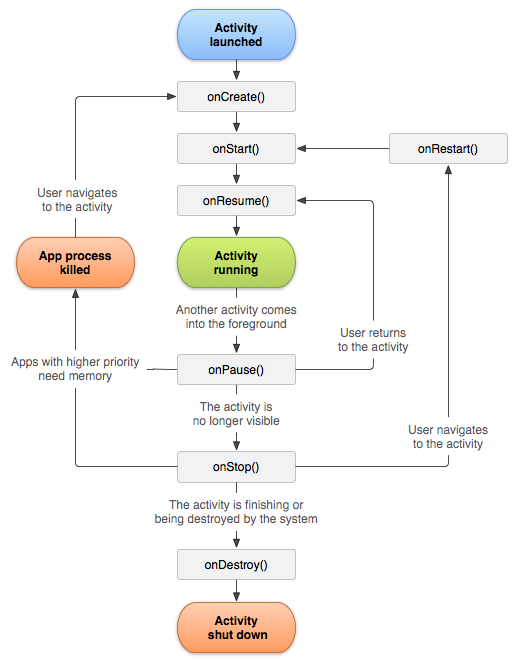
\includegraphics[scale=.33]{./img/activityLifecycle.png}
\end{figure}
\end{block}
\end{frame}

\begin{frame}[fragile]{Hola Mundo}
\begin{block}{}
\textbf{./res/layout/activity\_main.xml}
\begin{xmlcode}
<RelativeLayout
    android:layout_width="match_parent"
    android:layout_height="match_parent"
    tools:context=".MainActivity" >
    <TextView
        android:layout_width="wrap_content"
        android:layout_height="wrap_content"
        android:text="@string/hello_world" />
</RelativeLayout>
\end{xmlcode}
\textbf{./res/values/strings.xml}
\begin{xmlcode}
<resources>
    <string name="hello_world">Hello world!</string>
</resources>
\end{xmlcode}
\end{block}
\end{frame}
% Placing a * after \section means it will not show in the
% outline or table of contents.
\section*{Qué hemos visto}

\begin{frame}{Qué hemos visto}
  \begin{itemize}
  \item
    Cómo preparar el entorno para desarrollar aplicaciones Android.
  \item
    Conceptos básicos Android.
  \item
    Creación de un proyecto Hola Mundo.
  \end{itemize}
\end{frame}

\begin{frame}{¿Y ahora qué?}
  \begin{itemize}
  \item
    A partir de ahora, trabajaremos sobre ejemplos funcionales, deteniéndonos en las partes de código importantes para explicarlas.
  \end{itemize}
\end{frame}
